\section{Extensions}\label{sec:extension}

In this section, we present two extensions to our generalize our algorithms and theoretic analysis. First, we investigate the adaptation of Algorithm \ref{alg:nested_wait} to accommodate time-varying arrival rates. Second, we propose a generalized segment design for Algorithm \ref{alg:nested_wait}, extending beyond the existing $m$-segment parameterization. We establish that these extensions preserve comparable theoretical guarantees as in Theorem \ref{thm:nested_wait_heavy_traffic}.

\subsection{Time-Varying Arrival Rates}\label{sec:time_varying}

In this part, we analyze the asymptotic optimality of the Nested WAIT algorithm under time-varying arrival rates, denoted $\lambda_j^t$ for prompt type $j \in [m]$ at time $t \in [0, T]$. We assume that $\lambda_j^t$ are continuous functions of time, uniformly bounded by $\lambda_{\max} < \infty$. Define the accumulated arrivals of type $j$ over the interval $[t_1, t_2]$ as $\lambda_j[t_1, t_2] := \int_{t_1}^{t_2} \lambda_j^t \, dt$. Recall from Equation \eqref{eq:wait_thresholds} that $\Delta T_{[1,2,\dots,m]}(n_1,\cdots,n_m)$ represents the per-iteration time cost when processing exactly $n_i$ prompts at each stage in segment $i$, for all $i \in [m]$, as \eqref{eq:nested_wait_thresholds} ($n_i$ is the threshold defined in Algorithm \ref{alg:nested_wait}).

For the Nested WAIT policy defined by $\pi = [n_1, \dots, n_m]$, we consider the following conditions for all $t\in [0, T]$, $0<\Delta t\leq \Delta T_{[1,2,\cdots,m]}(n_1,\cdots,n_m)$ and $i = 1, 2, \dots, m-1$, analogous to \eqref{eq:nested_wait_thresholds}:
\begin{equation}
    \label{eq:nested_wait_thresholds_time_varying}
\begin{aligned}
        & \sum_{j=1}^m \lambda_j\big[t, t + \Delta t\big] \\&\leq \sum_{j=1}^m \lambda_j\big[t, t +\Delta T_{[1,2,\cdots,m]}(n_1,\cdots,n_m)\big]< n_1, \\
        & n_{i+1}/n_i > p_i[t,t+\Delta t],
    % & n_{i+1} \sum_{j=i}^m \lambda_j\big[t, t + \Delta t \big]  > n_i \sum_{j=i+1}^m \lambda_j\big[t, t + \Delta t \big],.
\end{aligned}
\end{equation}
where $p_i[t,t+\Delta t] = (\sum_{j=i+1}^m\lambda_j[t,t+\Delta t])/(\sum_{j=i}^m\lambda_j[t,t+\Delta t]).$

% Analogous to Equation \eqref{eq:nested_wait_thresholds}, we consider thresholds satisfying:
% \begin{equation}
%     \label{eq:nested_wait_thresholds_time_varying_ineq}
%     \Delta T_{[1,\dots,m]}(n_1,\dots,n_m) < \frac{n_1}{\sum_{j=1}^m \lambda_j(s)}, \quad 
%     \frac{n_{i+1}}{\sum_{j=i+1}^m \lambda_j(s)} > \frac{n_i}{\sum_{j=i}^m \lambda_j(s)}, \quad \forall i = 1, 2, \dots, m-1, \; \forall s \in \mathbb{N}.
% \end{equation}
 We define that the total number of iterations over time horizon $[0,T]$ as $ S$. Therefore, we have $T\ge\sum_{s=1}^S \Delta T_{s\text{-th Batch}}\geq S\cdot \min \Delta T_{\text{Batch}}$, where $ \Delta T_{s\text{-th Batch}}$ denotes the time cost of the $s$-th iteration and $\Delta T_{\min}=\min_s\{\Delta T_{\text{Batch}}\}$.
We now present the following result that extends Theorem \ref{thm:nested_wait_heavy_traffic}.

\begin{theorem}
\label{thm:nested_wait_heavy_traffic_time_varying}
Suppose the thresholds $\pi = [n_1, \dots, n_m]$ satisfy \eqref{eq:nested_wait_thresholds_time_varying}, and the memory $M^{(\zeta,\pi)}$ fulfills:
\[
\begin{aligned}
M^{(\zeta,\pi)}
&\geq M^{\pi} + \sum_{j=2}^m (l + l_{j-1}') \left(n_j + \theta_j^{-1} \ln\!\left( \tfrac{m \zeta S}{\delta} \right)\right) \\
&= O\!\left( 2M^\pi + \sum_{j=1}^m \theta_j^{-1}  (l + l_{j-1}') \ln\!\left( \tfrac{m \zeta S}{\delta} \right) \right),
\end{aligned}
\]
where the memory usage $M^\pi$ is defined as \eqref{eq:nested_wait_memory} and $\theta_j$ is given in (\ref{eq::eq of theta, time varying}) with the lower bound in Equation (\ref{eq::theta lower bound}). Then, the following asymptotic bounds hold:
$$
    \begin{aligned}
        &\throughput^* - \mathbb{E}\left[ \throughput^{(\zeta, \pi)} \right] 
   = O\left( (\zeta T)^{-1} \right), \\
&\mathbb{E}\left[ \Latency^{(\zeta, \pi)} \right], \,\mathbb{E}\left[ \TTFT^{(\zeta, \pi)} \right] = O(1).
    \end{aligned}
$$
Additionally, the memory usage remains below $M^{\zeta,\pi}$ with probability at least $1 - \delta$ over the time hotizon $[0,T].$
% total batch counts $s\in \{1,\cdots,S\}$ in time horizon $[0,T]$, bounded by $S \le T=\sum_{i=1}^S \Delta T_{i\text{-th Batch}}  /\min \Delta T_{\text{Batch}}$.
\end{theorem}

The proof constructs a coupled dominant stochastic process, extending the approach of Theorem \ref{thm:nested_wait_heavy_traffic} with adjustments for time-varying arrival rates. A detailed proof is provided in Appendix \ref{appendix:: proof of nested optimality, time varying.}.

\subsection{Segment Design}

In this subsection, we generalize the segment design in Algorithm \ref{alg:nested_wait}. We assume constant arrival rates, though the approach can be extended to time-varying rates as discussed earlier. Consider $m$ prompt types with decode lengths $l_1' < \cdots < l_m'$ and arrival rates $\lambda_1, \lambda_2, \cdots, \lambda_m$. Our objective is to merge these into $L$ segments, where $L \leq m$. For notational convenience, let $\Delta L:= m/L$. We partition the $m$ types into $L$ segments as follows: types $1$ to $\Delta L$, types $\Delta L+ 1$ to $2\Delta L$, $\dots$, types $(L-1)\Delta L+ 1$ to $m$.

For each segment $i \in \{1, \dots, L\}$, the total arrival rate is defined as $\lambda_i' = \sum_{(i-1)\Delta L+1\le j\le i\Delta L} \lambda_j$. Additionally, we define $\lambda'(i_1 \to i_2) := \sum_{j=i_1}^{i_2} \lambda_j'$ for $1 \leq i_1 \leq i_2 \leq L$.

Given a policy $\pi=[n_1,\dots,n_L]$ with threshold $n_i$ for the $i$-th segment in Algorithm \ref{alg:nested_wait}, we formulate a linear system analogous to Equation \eqref{eq:nested_wait_thresholds}:
\begin{equation}          \label{eq:nested_wait_thresholds_L}
    \begin{aligned}
    &\Delta T_{[1:L]}(n_{1:L}) \leq \frac{n_1}{\sum_{j=1}^L \lambda_j'},  \\
    &\frac{n_{i+1}}{n_i} > p_i, \ \forall i < L,
    \end{aligned}
\end{equation}
where $p_i =\frac{\lambda'(i+1 \to L)}{\lambda'(i \to L)}$, $\Delta T_{[1,\dots,L]}(n_1,\dots,n_L) = d_0 + d_1 M^\pi(n_1, \dots, n_L)$, and the  memory $M^\pi$ running with $n_i$ at each stage in segment $i$ is given by:
\[
M^{\pi}(n_1, \dots, n_L) = \sum_{i=1}^L n_i \left( l + \frac{i}{2} \Delta L\right) \Delta L.
\]

 We define that the total number of iterations over time horizon $[0,T]$ as $ S$. Therefore, we have $T\ge\sum_{s=1}^S \Delta T_{s\text{-th Batch}}\geq S\cdot \min \Delta T_{\text{Batch}}$, where $ \Delta T_{s\text{-th Batch}}$ denotes the time cost of the $s$-th iteration and $\Delta T_{\min}=\min_s\{\Delta T_{\text{Batch}}\}$. We demonstrate that the Nested WAIT algorithm (Algorithm \ref{alg:nested_wait}) with $L$ segments and thresholds $[n_1, \dots, n_L]$ satisfying Equation \eqref{eq:nested_wait_thresholds_L} achieves asymptotic optimality under the heavy-traffic conditions outlined in Section \ref{sec:nested_wait}.

\begin{theorem}
\label{thm:nested_wait_heavy_traffic, any segment}
For any fixed number of segments $L$ and thresholds $\pi = [n_1, \dots, n_L]$ satisfying Equation \eqref{eq:nested_wait_thresholds_L}, if the memory capacity $M^{(\zeta, \pi)}$ satisfies:
\begin{equation}
    \label{eq:nested_wait_memory_L}
    \begin{aligned}
M^{(\zeta, \pi)} 
&\geq M^\pi 
+ \sum_{j=2}^L (l + l_{j-1}') n_j \\
&\quad 
+ \sum_{j=2}^L (l + l_{j-1}') \theta_j^{-1} 
\ln\left( \frac{m \zeta S}{\delta} \right) \\
&= O\biggl( 2M^\pi 
+ \sum_{j=1}^L (l + l_{j-1}') \theta_j^{-1}
\ln\left( \frac{m \zeta S}{\delta} \right) \biggr),
    \end{aligned}
\end{equation}
where $\theta_j$ is given by Equation (\ref{eq::eq of theta}) with lower bound $8(n_j-n_{j-1}p_j)/n_j..$
% in Equation (\ref{eq::theta lower bound})
, then the performance of Nested WAIT is guaranteed by:
\[ 
    \begin{aligned}
        \throughput^* 
- \mathbb{E}\left[ \throughput^{(\zeta, \pi)} \right] 
&= O\left( (\zeta T)^{-1} \right), \\
\mathbb{E}\left[ \Latency^{(\zeta, \pi)} \right] ,\,\mathbb{E}\left[ \TTFT^{(\zeta, \pi)} \right] 
&= O(1).
    \end{aligned}
\]
Moreover, memory is not exceeded with probability at least \( 1 - \delta \) over the total batch counts $s\in \{1,\cdots,S\}$ as well as the time horizon $t \in [0, T]$.
% , where the total time horizon $T=\sum_{i=1}^S \Delta T_{i\text{-th Batch}}\geq S\cdot \min \Delta T_{\text{Batch}}$.
\end{theorem}

The proof follows a similar structure to that of Theorem \ref{thm:nested_wait_heavy_traffic}, substituting the original arrival rates $(\lambda_1, \dots, \lambda_m)$ with the clustered rates $(\lambda_1', \dots, \lambda_L')$ as in Appendix \ref{appendix::proof of nested_wait_heavy_traffic}. We omit here for simplicity.

To show how the memory requirements in \eqref{eq:nested_wait_memory_L} varies with different model parameters, we utilize the dataset from \cite{zheng2023lmsys} (Section \ref{sec:experiments}), with $m = 500$ prompt types, decode lengths ranging from 1 to 500, and a fixed prefill length of 62. The distribution of prompt types is shown in Figure \ref{fig:lambda_list}, where arrival rates are set proportional to normalized frequencies.

\begin{figure}[ht]
    \centering
    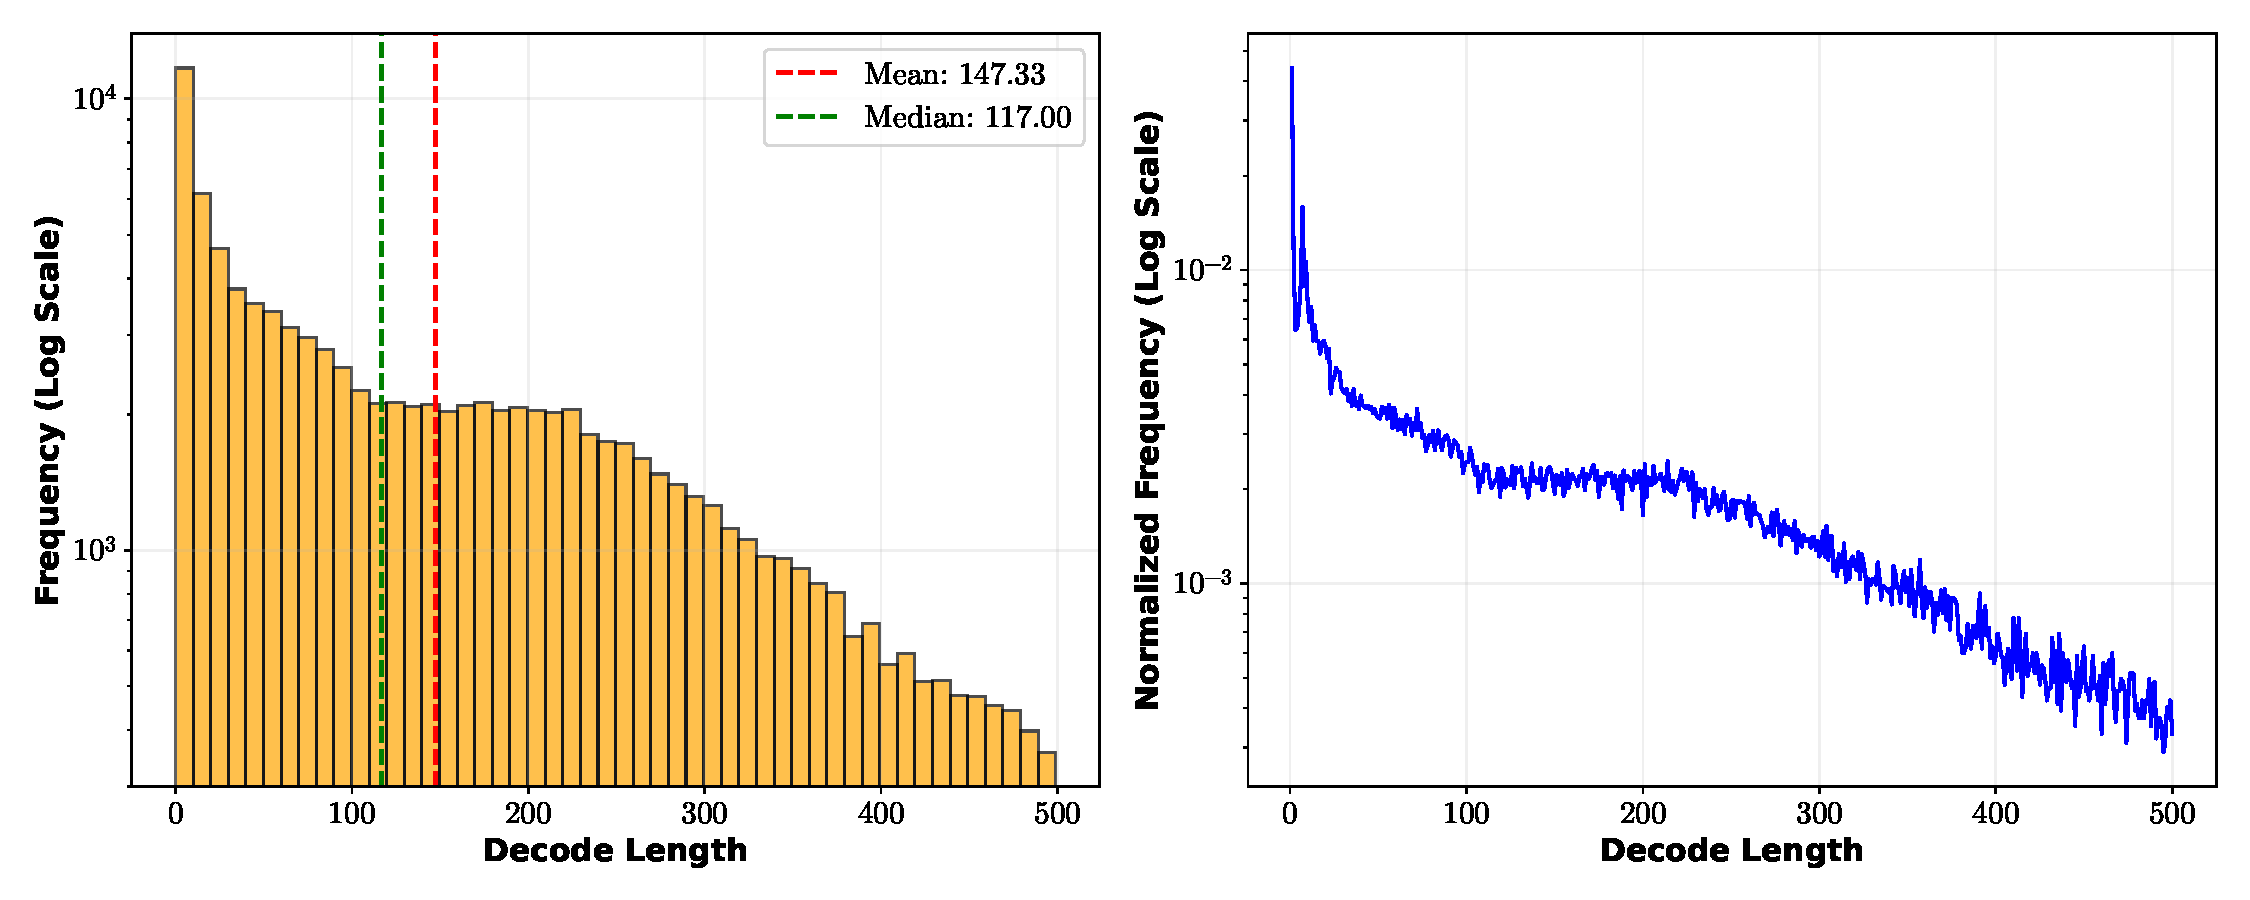
\includegraphics[width=0.8\textwidth]{Experiments_pdf/lambda_list.pdf}
    \caption{Arrival rate construction from real data, with rates proportional to normalized frequencies.}
    \label{fig:lambda_list}
\end{figure}

We analyze the three components of the memory bound in Equation \eqref{eq:nested_wait_memory_L}: (1) the peak batch memory usage $\sum_{j=1}^L n_j \left( l + \frac{j}{2} \Delta \right) \Delta$, (2) the queue length bound $\sum_{j=2}^L n_j (l + l_{j-1}')$, and (3) the high-probability queue length bound $\sum_{j=2}^L \theta_j^{-1} (l + l_{j-1}') \ln\left( \frac{(L - 1) (T + 1)}{\delta} \right)$.

Simulations under varying total arrival rates, time horizons $T$, and confidence levels $\delta$ are presented in Figures \ref{fig:fixed_T_200_rate_50_delta_0.1_1e-5}, \ref{fig:fixed_T_200_rate_500_delta_0.1_1e-5}, and \ref{fig:fixed_delta_0.001_rate_50_T_20_2000}. These figures depict the memory usage proportions of the three terms across different segment numbers $L$, revealing that the overall memory demand is primarily driven by the first term (fluid equilibrium memory) and follows a U-shaped trend with respect to $L$, suggesting that moderate segment number can reduce waste of memory usage. Additionally, Nested WAIT effectively manages unknown prompt types with only a marginal increase in memory beyond the fluid equilibrium requirement. In practice, a moderate number of segments, such as $L = 10$ as used in Section \ref{sec:experiments}, is sufficient.

\begin{figure}[ht]
    \centering
    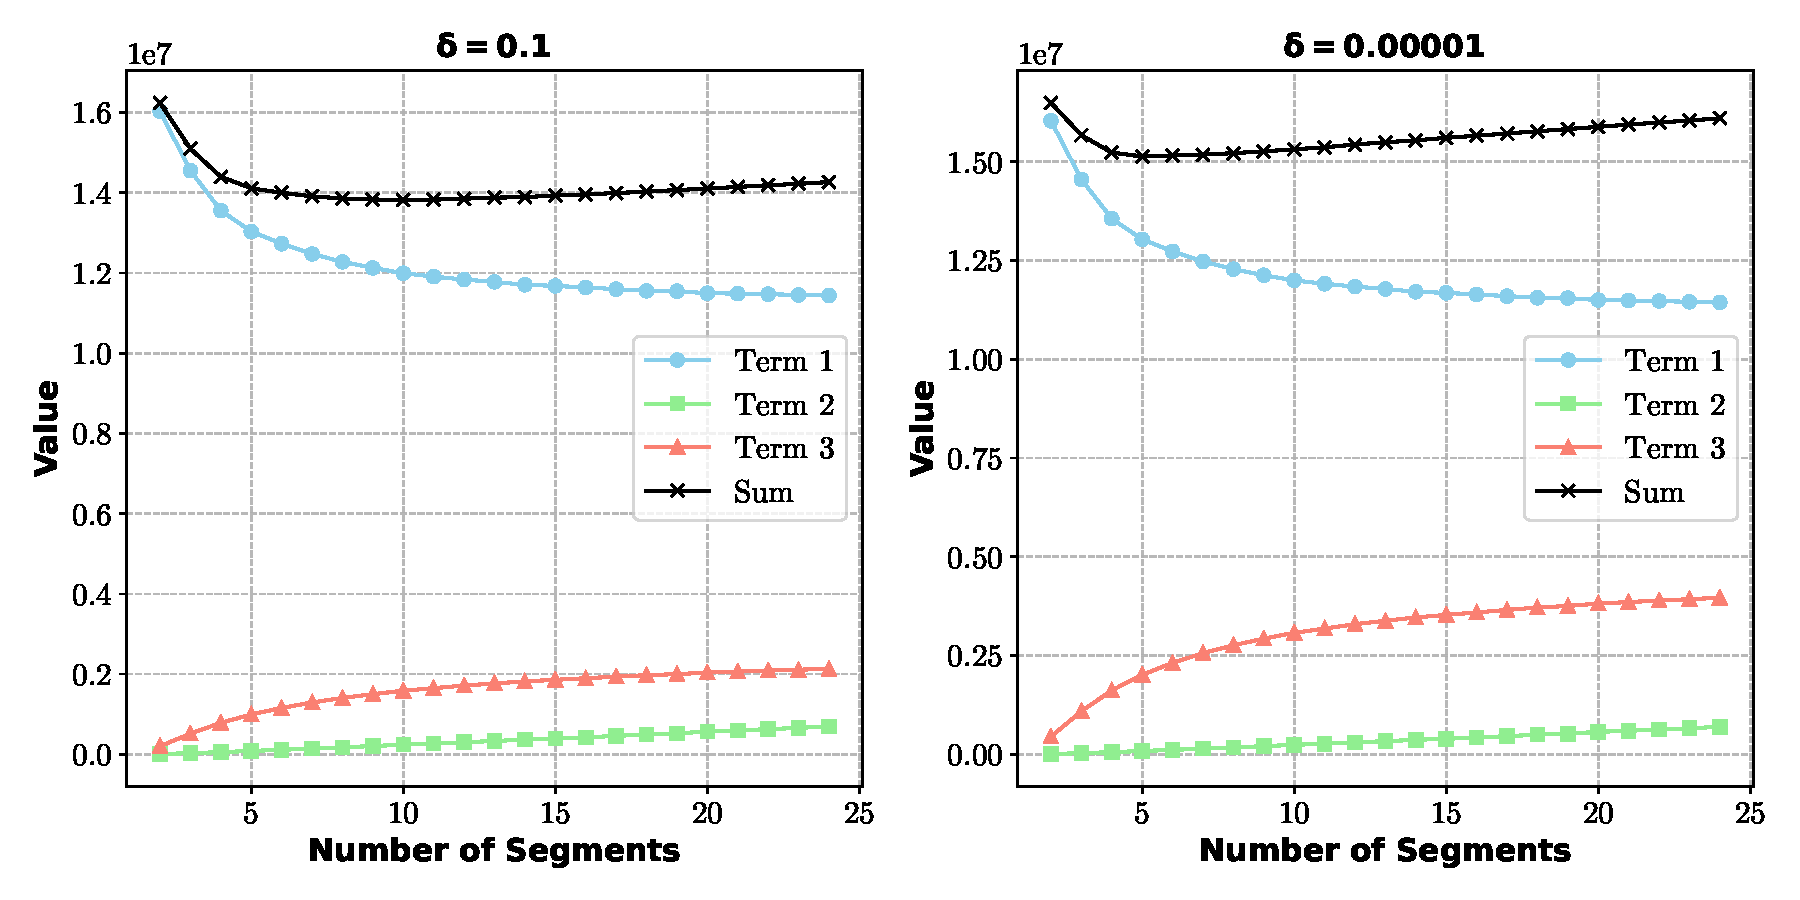
\includegraphics[width=0.8\textwidth]{Experiments_pdf/total_rate=50,T=200.pdf}
    \caption{Memory usage proportions under low arrival rate (total rate = 50, $T = 200$). Left: $\delta = 0.1$; Right: $\delta = 10^{-5}$.}
    \label{fig:fixed_T_200_rate_50_delta_0.1_1e-5}
\end{figure}

\begin{figure}[ht]
    \centering
    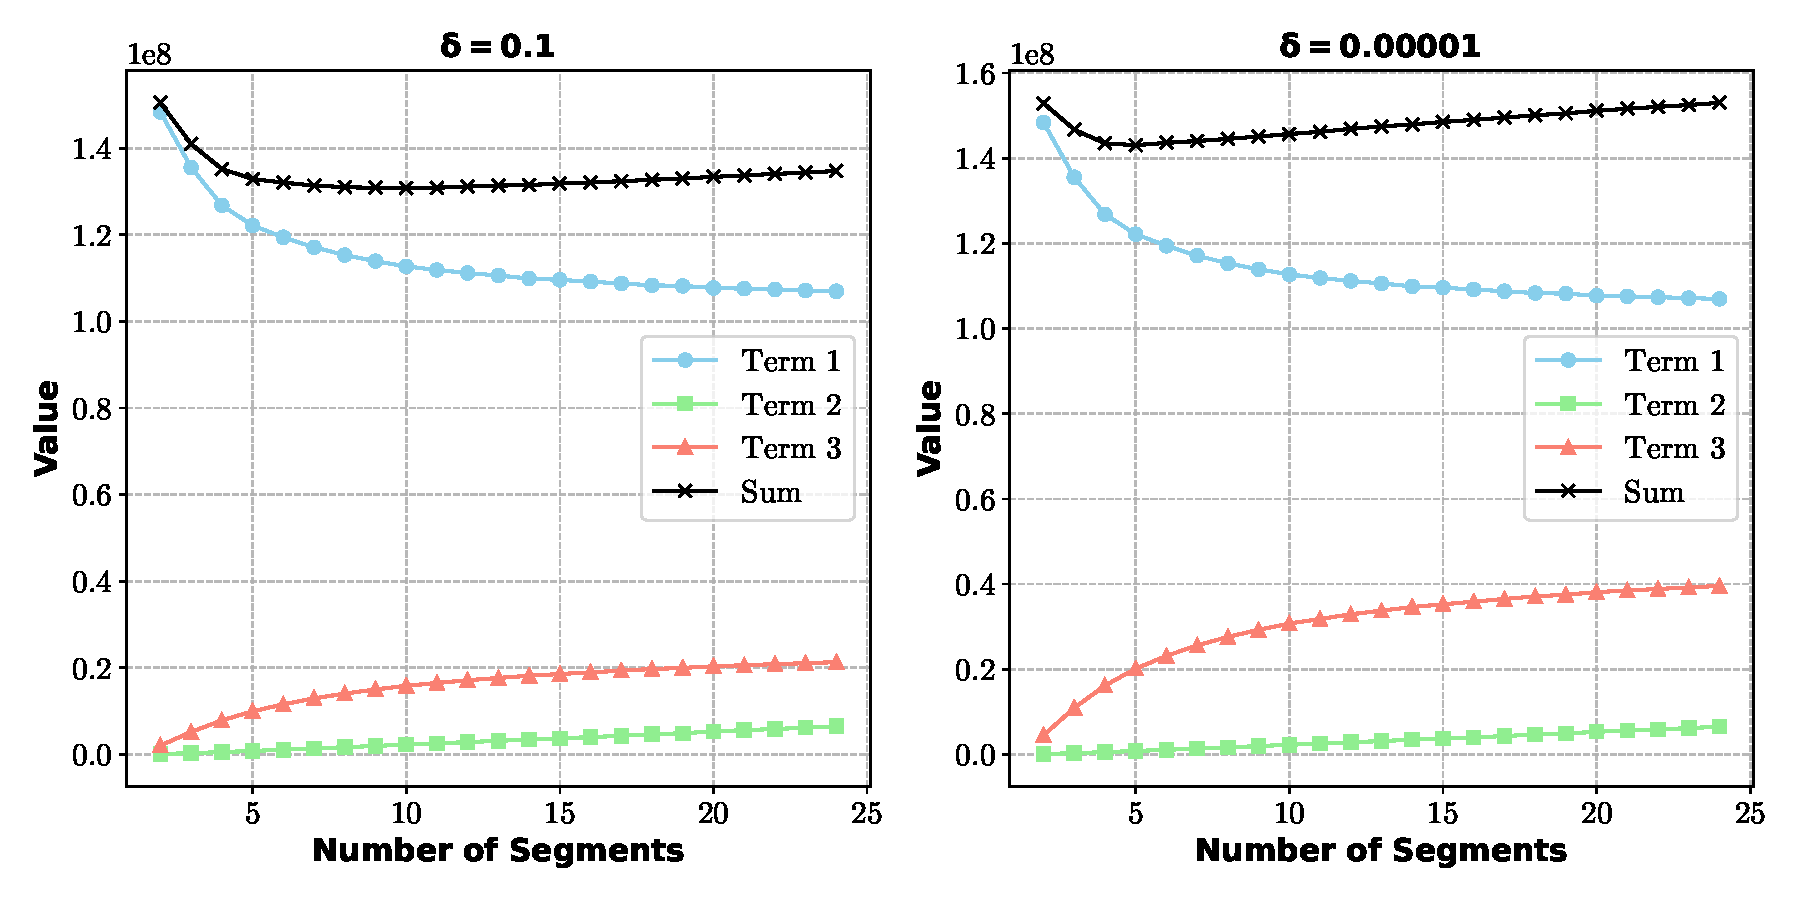
\includegraphics[width=0.8\textwidth]{Experiments_pdf/total_rate=500,T=200.pdf}
    \caption{Memory usage proportions under high arrival rate (total rate = 500, $T = 200$). Left: $\delta = 0.1$; Right: $\delta = 10^{-5}$.}
    \label{fig:fixed_T_200_rate_500_delta_0.1_1e-5}
\end{figure}

\begin{figure}[ht]
    \centering
    
\includegraphics[width=0.8\textwidth]{Experiments_pdf/total_rate=50,delta=0.001,T=20or2000.pdf}
    \caption{Memory usage proportions with varying time horizons (total rate = 50, $\delta = 0.001$). Left: $T = 20$; Right: $T = 2000$.}
    \label{fig:fixed_delta_0.001_rate_50_T_20_2000}
\end{figure}

% \subsection{Different prefill length}
% For the analysis of Nested WAIT, we assume that the prefill lengths of different prompts are all $l$.



% \subsection{Optimality under arbitrary segments}
% \gan{Maybe this subsection should be put later.}

